%\documentclass[acmjacm,acmnow]{acmtrans2m}
%\documentclass[conference,final]{IEEEtran}
%\documentclass[10pt,letterpaper]{article}
\documentclass[preprint,12pt]{article}

\usepackage{graphicx}
\usepackage{url}
\usepackage{color}
\usepackage{pdfsync}

% \acmVolume{}
% \acmNumber{}
% \acmYear{}
% \acmMonth{}


%\usepackage{sectsty}
%\usepackage{setspace}

% \usepackage{ifpdf}
% \usepackage{wrapfig}
% %\usepackage[cm]{fullpage}
% \usepackage{textcomp}
% \usepackage{srcltx}
% \usepackage{fancyhdr}
% \usepackage{setspace}
\usepackage{lscape}
% \usepackage{longtable}
% \usepackage{paralist}

%\usepackage{hyperref}
%\usepackage{pdfsync}

% \usepackage{ams}

% \ifpdf    %   \usepackage[pdftex,
%               colorlinks=true,
%               linkcolor=red,
%               citecolor=red,
%               filecolor=red,
%               ]{hyperref}
% \else
%   \usepackage[hypertex]{hyperref}
% \fi

% Space saving
%\usepackage[small,compact]{titlesec}
%\usepackage[small,it]{caption}

% \renewcommand\floatpagefraction{.9}
% \renewcommand\topfraction{.9}
% \renewcommand\bottomfraction{.9}
%\renewcommand\textfrare{.1}

\setcounter{totalnumber}{50}
\setcounter{topnumber}{50}
\setcounter{bottomnumber}{50}

%\textwidth = 6in
%\textheight = 8.5 in
%\oddsidemargin = 0.0 in
%\evensidemargin = 0.0 in

% \topmargin = 0.0 in
% \headheight = 0.0 in
% \headsep = 0.0 in
%\parskip = 0.0in
%\parindent = 0.5cm
\parskip = 0.04in
% \parindent = 0.0cm
% \textfloatsep = 0.1in

% \usepackage[draft,pdftex,colorlinks=true, linkcolor=blue,citecolor=blue,
%        urlcolor=blue]{hyperref}

% \ifpdf
% \pdfinfo{ /Author (Shantenu Jha et al.)  /Title (Programming Abstractions for Large-Scale Distributed Applications) }
% \fi

\newcommand{\projectnamefull}{\textit{Programming Abstractions for
    Large-Scale Distributed Applications} }

\newcommand{\upup}{\vspace*{-0.5em}}
\newcommand{\up}{\vspace*{-0.25em}}
\newcommand{\I}[1]{\textit{#1}}
\newcommand{\B}[1]{\textbf{#1}}
\newcommand{\T}[1]{\texttt{#1}}
\newcommand{\BI}[1]{\B{\I{#1}}}

% \ifpdf
%   \DeclareGraphicsExtensions{.pdf, .png, .jpg}
% \else
%   \DeclareGraphicsExtensions{.ps, .eps}
% \fi

\long\def\comment#1{{\bf \textcolor{magenta}{\bf #1}}}
\long\def\ccomment#1{{\bf \textcolor{blue}{\bf #1}}}
\newcommand{\C}{\comment}
\newcommand{\CC}{\ccomment}

\newcommand{\yes}{$\bullet$}

\long\def\finalcomment#1{{\bf \textcolor{red}{\bf #1}}}
\newcommand{\CF}{\finalcomment}

\newif\ifdraft
\drafttrue
\ifdraft
 \newcommand{\katznote}[1]{ {\textcolor{magenta}    { ***Dan:      #1 }}}
 \newcommand{\rananote}[1]{ {\textcolor{blue}    { ***Omer:     #1 }}}
 \newcommand{\note}[1]{ {\textcolor{red}    { #1 }}}
\newcommand{\manishnote}[1]{{\textcolor{green}   { ***Manish:   #1 }}}
\newcommand{\jhanote}[1]{  {\textcolor{blue}     { ***Shantenu: #1 }}}
 \newcommand{\jonnote}[1]{  {\textcolor{red}      { ***Jon: #1 }}}
\else
 \newcommand{\katznote}[1]{}
 \newcommand{\rananote}[1]{}
 \newcommand{\note}[1]{}
 \newcommand{\manishnote}[1]{}
 \newcommand{\jhanote}[1]{}
 \newcommand{\jonnote}[1]{}
\fi

\title{3DPAS: Distributed Dynamic Data-intensive Programming
  Abstractions and Systems}

%\author{J.D. Blower$^{10}$, Neil Chue-Hong$^{}$, Simon Dobson$^{}$,
%  Shantenu Jha$^{1,2,3}$, Daniel S. Katz$^{4,1,5}$, Omer Rana$^{8}$}

\author{ Shantenu Jha, J.D. Blower, Neil Chue-Hong, \\[-0.1em]
Simon Dobson, Daniel S. Katz, Omer Rana}

%Manish Parashar$^{6,7}$,
%   Jon Weissman$^{9}$,

%   \small $^1$Center for Computation \& Technology,
%   Louisiana State University\\[-0.1em]
%   \small $^2$Department of Computer Science,
%   Louisiana State University\\[-0.1em]
%   \small $^3$e-Science Institute,   University of Edinburgh\\[-0.1em]
%   \small $^4$Computation Institute,   University of Chicago\\[-0.1em]
%  \small $^5$Department of Electrical and Computer Engineering,
%   Louisiana State University\\[-0.1em]
%   \small $^6$NSF Center for Autonomic Computing, Rutgers University\\[-0.1em]
%   \small $^7$Department of  Electrical and Computer Engineering, Rutgers University\\[-0.1em]
%   \small $^8$Department of Computer Science,
%   Cardiff University\\[-0.1em]
%   \small $^9$Department of Computer Science,
%   University of Minnesota\\[-0.3em]
%   \small $^10$Reading e-Science Centre, University of Reading, UK
%}
\begin{document}
\maketitle

\begin{abstract}
  Many problems at the forefront of science, engineering, medicine,
  and the social sciences, are increasingly complex and
  interdisciplinary due to the plethora of data sources and
  computational methods available today.  A common feature across many
  of these problem domains is the amount and diversity of data and
  computation that must be integrated to yield insights. Such data is
  increasingly large-scale and distributed;
  the data-sets, their location and scheduling decision
  are time-dependent. % Applications need access
  % to these disparate data-sets and to the methods that operate on
  % them.  Data-intensive applications need first-class support for
  % distributed heterogeneous platform execution.
  The 3DPAS Research theme (funded by the eSI, Edinburgh and US NSF),
  aims to investigate applications that have these characteristics, in
  other words it operates at the triple point of {\it dynamic} and
  {\it distributed} and {\it data-intensive}, (3D) attributes.  This
  evolving document represents work in progress of the 3DPAS Research
  Theme.
\end{abstract}

%\input{notes}

\section{Introduction: Context, Scope and Outline}

\jhanote{Overall introduction, leading into some specific examples.}


\section{Understanding Distributed Dynamic Data}

Why bother about distributed, dynamic and data-intensive applications?
\jhanote{(Shantenu, Omer, Neil, Simon, and Dan)}

\subsection{Importance of Distributed}

\subsection{Importance of Dynamic and Examples}

There is a general appreciation that the challenges of data-intensive
applications span beyond large-volumes and management/curation.  One
specific attribute that we believe is pervasive but not necessarily
obvious is “dynamic data”. The belief is based upon the fact that data
is often distributed, and as a consequence many attributes of
distributed systems permeate to data. Additionally the requirement of
many applications impose a requirement that data is dynamic.

\subsection{Types of Dynamic Data}
Some example of such dynamism:

\begin{itemize}
\item Change of data operated upon.
\item Variability of data rate -- arrival, consumption or ability to generate (due to dependencies)
\item Data placement and scheduling issues are time dependent
\item The nature of coordination between the different execution units
changes
\end{itemize}

\jhanote{Possibly merge?}

\begin{enumerate}

\item Streaming data -- data comes and goes
  \url{http://traffic.berkeley.edu/} and
  \url{http://lagrange.ce.berkeley.edu/fsn/}
\item Data set that is being operating upon is changing
\item Data has to be transformed
\item Placement decisions time-dependent
\end{enumerate}

\jhanote{We should highlight which of the above dynamic case are to be
  found in applications}

\katznote{Question: is there anything unique about scientific work on
  streaming data?  Or is all work on streaming data basically them
  same, whether it's in science or finance, for example?}

\jhanote{Good Q: I think other than scale -- of data volume, and
  degree of variability they are not too dissimilar}

\subsection{Characterising Dynamic Applications}

Amdahl’s number has been useful in characterising “static”
data-intensive applications and systems. We believe there is scope to
generalize Amdahl’s number to capture attributes of dynamic data
applications.

\subsubsection{Dynamic Data in a Web Environment}

The NERC\footnote{UK Natural Environment Research Council} Virtual
Observatory\footnote{http://www.nerc.ac.uk/research/programmes/virtualobservatory/}
is a new initiative to create a pilot cloud-based environment in which
different practitioners will discover, visualize and process data
relating to the UK's system of rivers and soils.  It will provide
access to many different kinds of distributed hydrological data,
including sensor data and numerical models, many of which produce
rapidly-changing, dynamic information.  There are many scientific
challenges to be faced, notably including the coupling of the models
and observations; this includes the possibility that sensors can be
dynamically tasked in response to model forecasts, or that models may
adapt dynamically to new information from sensors.  Principles of the
Web and ``linked data'' may help to solve some of the challenges in
informatics, but many technical challenges will remain regarding the
handling of dynamic data, including keeping careful records of its
provenance in order to record the steps taken in making a decision.

\emph{Just some placeholder notes from Jon.  Could belong elsewhere.}

Web Services are commonly used to distribute data through HTTP.  A key
characteristic of dynamic data, of course, is that it changes with
time.  It is of great importance for the user to be confident that she
is accessing the correct version of the data; this will often be the
most up-to-date data, or may be a specific historical version.  In a
Web environment, servers and proxy servers (which are sometimes beyond
the control of the data provider or the data user) may retain caches
of data in a strategy to reduce server load and network traffic.  For
this reason, the HTTP protocol provides mechanisms for defining expiry
times for data resources, specifying when a resource ought to be
cleared from the cache.

In the environmental and geospatial communities the Open Geospatial
Consortium specifications are being widely adopted alongside existing
protocols such as OPeNDAP.  Unfortunately these protocols, although
built atop HTTP, do not make it easy for this versioning to be
implemented correctly.  The OPeNDAP protocol does not have the concept
of a dataset version, meaning that clients have no reliable or
efficient means to detect that a dataset has changed.  The OGC
protocols in general [TODO: look into this], \emph{do} provide
versioning at the level of the service endpoint, but provide no
information on when a resource should be considered expired.  Clients
are therefore forced to poll the server to check for updates.

Therefore we see that in a ``pull'' environment such as the Web, it is
necessary for servers to advertise not only the version of a resource,
but also the expiry time in order to handle dynamic data correctly.
The frequency of updates is also useful information for service
consumers.  Expiry times can be specified using the mechanisms of HTTP
(although this capability is often not used in practice), but resource
versioning and update frequency must be handled at a higher level.

[All this must be fairly well-known and almost certainly covered in
the literature, with the possible exception of the material on OPeNDAP
and OGC.  Any references we could cite?]

\subsection{Other points to cover}

\begin{itemize}
\item Lay out several scenarios first, and then formulate/define Dynamic Data
\item Dynamic: transformed by the workflow scenario (state is captured by immutable objects)
\item How does this differ from Scientific Databases
\item How does it relate to Scientific Data Management and Scientific data flow
\item Carve out the specifics of this theme -- and how it relates to such existing approaches (a diagram would be nice)
\item Underlying data model (operations) are highly domain specific -- make clear what can be domain specific and domain independent
\item Relationship to ``legacy''
\item Dynamic data can arise at different levels (application vs. middleware (infrastructure)). Identify which is the primary consideration here, and what is different.
\item Reference to EU 2030 Objectives (part of the Project Europe 2030
  Report) -- underpins ``Data Intensive Research'' from an EU
  perspective (strategy) + relate this to NSF ``CIF21'' vision
\end{itemize}

How does Dynamic Data relate to Distributed \& ``Big'' Data? Relate to
DPA and Malcolm et al.'s theme (Data Lifecycle, Complexity, etc)


\section{Application Scenarios} {\bf Dan, Shantenu (co-leads), All}

Application Scenario Characteristics for Dynamic Data (Various)

Identify: (1) what is the case scenario within the application; (2) what data is dynamic; (3)  how the data is being used in the context of each of these scenarios.

Currently trying to do this by asking the following questions:
\begin{enumerate}
\item What is the purpose of the application?
\item How is the application used to do this?
\item What infrastructure is used? (including compute, data, network, instruments, etc.)
\item What dynamic data is used in the application?
\begin{enumerate}
\item What are the types of data,
\item What is the size of the data set(s)?
\end{enumerate}
\item How does the application get the data?
\item What are the time (or quality) constraints on the application?
\end{enumerate}

\katznote{new suggested questions from Don Middleton: How much diverse data integration is involved?  how diverse is the data?}

\subsection{Silvia's Biosciences app: NGS, medical imaging (Silvia)\label{bioSilvia}}

\begin{itemize}
\item Infrastructure monitoring for the execution of workflows to
  manage failure
\item the application is sequence alignment (split data (this is where there is dynamic decision making) to execute the alignment in parallel)
\item DTI Imaging: two cases are interesting: DTI atlas (split, run, merge, split, merge - reduction from 10000 tasks to 1 output); PCA for classification of patients/control
\end{itemize}

\subsubsection{Silvia's contribution}

NGS sequence alignment on the AMC e-bioscience infrastructure

1. What is the purpose of the application?

The application performs analysis of DNA sequencing data for various goals in life science research, e.g., Mutation screening, Virus discovery, Genome-wide Associations (GWA), Linkage analysis, Comparison of bacterial genomes, microRNA expression and Exome sequencing. The data analysis is composed of various methods that are implemented by a bioinformatician, whereas the data is typically owned by the life scientist.

2. How is the application used to do this?

Note: Here we focus on data analysis from the perspective of the bioinformatician, excluding steps related to data acquisition (transformation of raw images into sequences of amino acids) and posterior biostatistics and epidemiological analysis.

The data analysis is implemented as a pipeline of generic and customized components, mostly third-party public software tools. The pipeline may differ for each specific study, depending on the data acquisition and the research question. Typically it includes data preparation (file conversion, reformatting and filtering); alignment (comparison) with some reference database as the human genome; post-processing (output conversion, reformatting, statistical analysis) and visualization. Sequence alignment is the most computing-intensive step, which became prohibitive for sequential execution in next generation sequence experiments. All data is stored in files that are often completely read in memory for fast processing. Compressed formats are usually adopted. Although the files are large, the data can be easily decomposed because the processing is done on each sequence (`string') at a time.


3. What infrastructure is used? (including compute, data, network, instruments, etc.)

\begin{figure*}[htbp]
  \begin{center}
    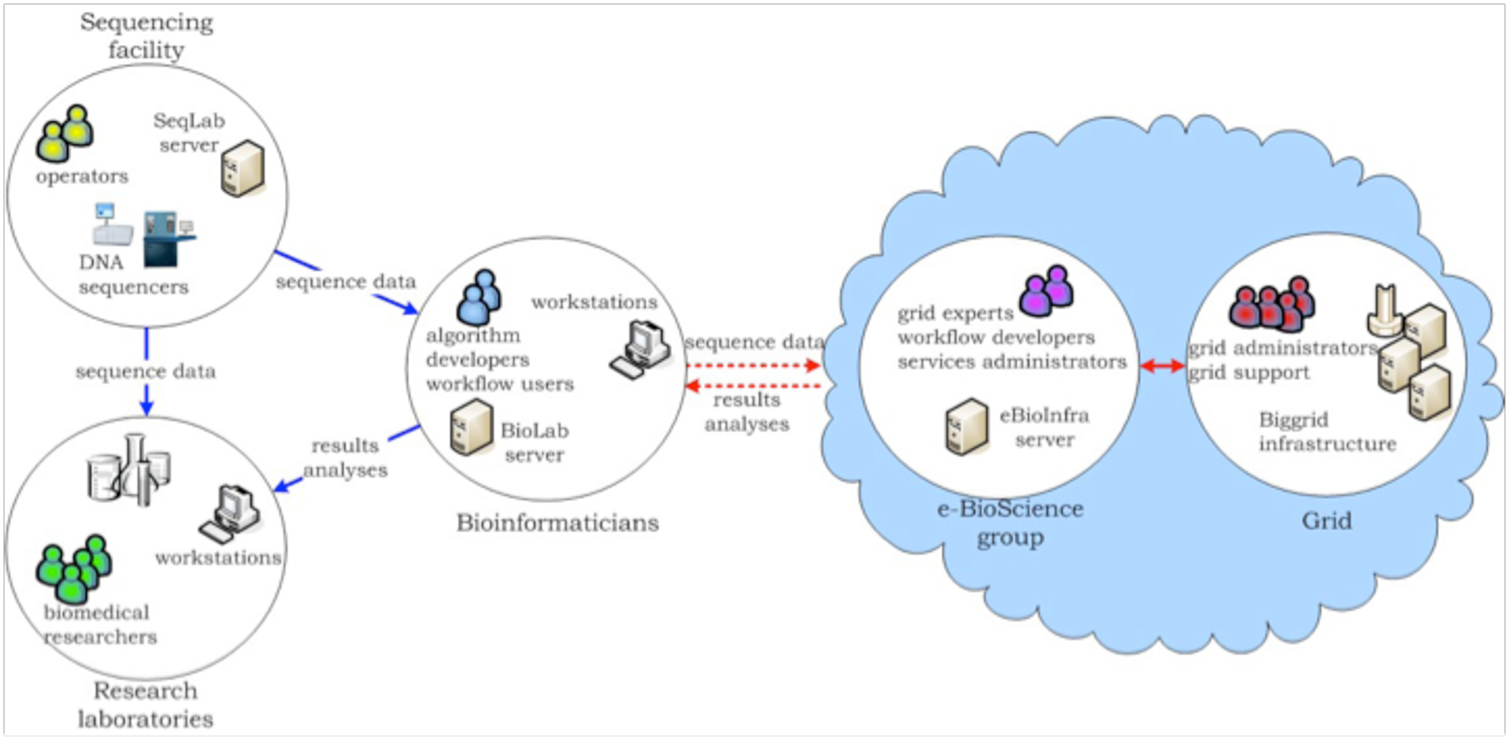
\includegraphics[width=\textwidth]{figures/silvia.pdf}
    \caption{Figure from Silvia}
    \label{Fig:silvia}
  \end{center}
\end{figure*}


see Figure~\ref{Fig:silvia}.

Data:

Data acquisition: Roche, Solid and Illumina next generation sequencers

Local storage: dedicated server at the AMC network (ftp)

Grid storage: Storage Elements of the Dutch e-Science Grid (www.biggrid.nl)

Data transport:

From sequencer to server: AMC network (XXX) or off-line media

Between data server and grid storage: public network (XXX);  lightpath (near future)

Between grid storage and worker nodes: public (XXX) or site (XXX) network

Computing:

Local Computing: clusters and servers at the AMC and workstations (laptops, desktops) anywhere
Grid Computing: Dutch Grid (www.biggrid.nl), part of EGI

Originally all steps were performed in some local server or on the user's workstation. The visualization is still performed in the user's (windows) workstation, but all the other steps are currently performed on the Dutch grid infrastructure. The pipeline is described as a grid workflow using the GWENDIA language (\url{http://dx.doi.org/10.1145/1645164.1645171}) and enacted on the Dutch Grid using the MOTEUR2 workflow engine (\url{http://modalis.polytech.unice.fr/softwares/moteur/start}).

PS: although only the alignment step is computation-intensive, it is more practical to perform all the others on the grid to minimize data transport to/from the user's workstation, which is normally on low speed networks. That is, the computation is statically and manually taken to the data in this case. This can lead to sub-optimal resource usage.

4. What dynamic data is used in the application?

Note: data is not really `dynamic' in this case -- the sequences are acquired once and analyzed many times. However the execution of this application on a distributed infrastracuture has dynamic aspects when optimized resource usage is considered:

\begin{itemize}
\item Split/merge the data according to available resources
\item Compute resource selection based on data location, processing profile and/or network capacity
\item Resource selection based on security constraints (access control, trust)
\item Collection and processing of monitoring information to steer grid enactment.
\end{itemize}

(a) What are the types of data,

DNA sequences (strings) stored in open formats (FASTA, SFF, SAM, BAM)
Bundles of results from alignment tools (custom format, binary?)

(b) What is the size of the data set(s)?

one example for BWA alignment tool (short sequences) follows:

input data: Sequencing Data in the csFasta format, normally 25-35~GB;
Quality files in the .qual format, normally 50-80~GB;
Reference DB in the Fasta BS format: 3.2~GB (human genome) 140~MB (one chromosome)

Intermediate files:
Reference BWA index, normally 4.5GB (human genome) 240~MB (one chromosome);
Sequencing Data in the FastQ format (fastq.gz), normally 20-30~GB

Output:
Results in .sai format (direct output of BWA), normally 2-3~GB;
Results in .sam format, normally 55-75~GB;
Results in .bam format, normally 20-30~GB

5. How does the application get the data?

From a local file. The legacy code is wrapped to stage the inputs and outputs in/out the worker node.

All data is stored in files that are often completely read in memory for fast processing. Compressed formats are usually adopted. Although the files are large, the data can be easily decomposed because the processing is done on each sequence (`string') at a time

6. What are the time (or quality) constraints on the application?

In research there are no strict constraints on the time to complete the analysis.
In patient care, time could determine life, death or money, but we have no concrete case yet.

Quality in this case refers to the accuracy of the results obtained. This is essential for research and patient care.




\subsection{WLCG (focus on ATLAS) (Steve Fisher) \label{WLCGSteve}}
\begin{itemize}
\item Most of the dynamism is in infrastructure, not in the application (e.g. use of PilotJob)
\item Application dynamism: location of file (e.g. if file turns out to be not local, look up in registry-- but not do this again)
\item No specific QoS issue concerned with data transfer times
\end{itemize}

\subsubsection{New answers from Steve}

3DPAS - Particle Physics - the example of Atlas physics channel selection.

   1.     What is the purpose of the application?

A physics group is interested in a specific physics channel (underlying physical process) as recorded by the Atlas experiment at the LHC (Large Hadron Collider) at CERN in Geneva. The set of available data grows steadily over time as more data are collected and reconstructed.

   2.    How is the application used to do this?

 Both physics groups and individuals run jobs as they see fit, either reading the reconstructed data or reading intermediate datasets created by themselves or their colleagues. If, in the future, resources should prove inadequate then adjustments to working practices to coordinate processing may be made to increase physics output.

   3.      What infrastructure is used? (including compute, data, network, instruments, etc.)

The WLCG (Worldwide LHC (Large Hadron Collider) Computing Grid) is used with a mixture of gLite software, experiment specific software and physics group specific software. WLCG has 250,000 cores distributed over 140 sites and with 100PB of disk. CERN is connected to the eleven `Tier 1' national sites by a dedicated optical network. This may be extended in the future.

   4.      What dynamic data is used in the application?

The data being processed can be considered as dynamic as it grows steadily as new raw data are collected and the basic reconstruction program is run to produce information about specific particles involved in a collision. This reconstruction is rerun periodically (two or three times per year is expected) as calibrations of the detector are improved. Reconstruction algorithms are also improved as are the physics groups' selection codes. One output of the reconstruction is `tag' data - summary information written to a database to facilitate event selection. This is not yet used very much. Calibration data are held on an RDBMS with Frontier/Squid front ends.

         a.             What are the types of data,

          The bulk of the data is individual event data at different stages of refinement. This is held in a in-house representation of C++ serialized objects. Though this format is not standard it is used by all LHC experiments.

         b.            What is the size of the data set(s)?

          Roughly 20~TB of data are collected every day. Multiple generations of processed data are kept. Many data files are replicated on multiple sites; this is done both by copying it to where it is likely to be useful and partly dynamically as the need arises.

   5.      How does the application get the data?

A copy of the file is made to the SE (Storage Element) at the site where the job will run. From there it is either copied to a local disk or read from the SE.

   6.      What are the time (or quality) constraints on the application?

If some data are missed during processing the only effect is a reduction of statistical precision in the final analysis. Accurate book keeping is important to know which data have been processed. If the selection code has been improved then naturally the physics groups would like to see the results as soon as possible.


%\subsubsection{Old answers from Steve}
%
%   1.       What is the purpose of the application?
%
%A physics group is interested in a specific physics channel (underlying physical process) as recorded by the Atlas experiment at the LHC (Large Hadron Collider) at CERN in Geneva. The set of available data grows steadily over time as more data are collected and reconstructed. It would not be efficient to allow individual physics groups to process this large volume of data in an uncoordinated manner as it requires reading all available data.
%
%   2.       How is the application used to do this?
%
%Physics groups register their analysis code to be run on the next scheduled analysis ``train''. The train leaves every two weeks and reads through all the data, runs the physics selection code of each group and writes out the selected events and output from the computation to produce relatively small data sets for each physics group. The groups then use these selections to perform more ad-hoc analysis.
%
%   3.      What infrastructure is used? (including compute, data, network, instruments, etc.)
%
%The WLCG (Worldwide LHC (Large Hadron Collider) Computing Grid) is used with a mixture of gLite software, experiment specific software and physics group specific software. WLCG has 250,000 cores distributed over 140 sites and with 100~PB of disk. There is no wide area dedicated network infrastructure.
%
%   4.      What dynamic data is used in the application?
%
%The data being processed can be considered as dynamic as it grows steadily as new raw data are collected and the basic reconstruction program is run to produce information about specific particles involved in a collision. This reconstruction is rerun periodically (two or three times per year is expected) as calibrations of the detector are improved. Reconstruction algorithms are also improved as are the physics groups' selection code. Calibration data are held on an RDBMS with Frontier/Squid front ends.
%
%         a           What are the types of data,
%
%          The bulk of the data is individual event data at different stages of refinement. The is held in a non-standard representation of C++ serialized objects.
%
%         b.             What is the size of the data set(s)?
%
%          Currently the reconstructed data (excluding copies) is about m TB and is growing at about  n TB per month. Many data files are replicated on multiple sites. This is done both by copying it to where it is likely to be useful and partly dynamically as the need arises.
%
%   5.       How does the application get the data?
%
%This is mostly by copying the file to where the job will run - though some remote file access is also used.
%
%   6.  What are the time (or quality) constraints on the application?
%
%If some data are missed during processing the only effect is a reduction of statistical precision in the final analysis. If the selection code has been improved then naturally the physics groups would like to see the results as soon as possible.
%
%
\subsection{Astrophysics -- Virtual Observatory (Bob) \label{astroBob}}
\begin{itemize}
\item Analysis of data to generate event streams $\rightarrow$ lead to the
  positioning of telescopes
\end{itemize}

\subsubsection{Answers from Bob}

I'll assume that the ``application'' in question is the sum of the two
activities, despite the fact that they are different in many respects,
and I'll try and distinguish between them where appropriate.

Let me know if you want clarification or further information - in some cases I wasn't quite sure what you were after.

1. What is the purpose of the application?

An increasingly important feature of astronomical research is the existence of
systematic sky surveys covering the whole sky (or large fractions thereof) in
many different wavebands. The principal outcome from these surveys are
astronomical source catalogues, which contain values for attributes
characterizing all the celestial sources detected in the sky survey dataset.
These are now typically implemented in relational databases, with SQL interfaces
implemented through web pages, and the principal goal of the Virtual Observatory
(VO) is to standardize access to these, and other astronomical data resources,
so that astronomers can readily perform multi-wavelength analyses, combining all
the extant data on particular sources.

      2. How is the application used to do this?

The VO includes a registry that contains metadata describing all the data
resources published using VO data access standards, enabling the discovery of
datasets relevant to a particular analysis. Web service implementations of data
access protocols enable users to access data in these repositories
programmatically, and distributed scratch space is provided for the storage of
intermediate result sets, so the user does not need to route large data flows
through his/her own workstation. In the future, more and more data analysis
software will be made available through web services compliant with VO
standards, enabling more of the data integration and analysis process to be
combined in workflow.

      3. What infrastructure is used? (including compute, data, network,
      instruments, etc.)

The data resources published to the VO exist in a number of data centers
distributed internationally. Major datasets---e.g. those from large sky
surveys---are typically implemented in relational databases running on high-spec servers
or clusters thereof. The compute requirements of the VO are currently modest,
but are likely to increase over time. Astronomers typically use normal academic
networks, but more specialized networking is required in some cases: e.g., sky
survey data is moved from Cambridge to Edinburgh using the UKLight project's
dedicated optical network, and radio interferometers require high-bandwidth
fibre connections from each antenna to the correlator.

      4. What dynamic data is used in the application?
(a) What are the types of data, (b) What is the size of the data set(s)?

The VO currently includes little dynamic data. The one exception is VOEvent
messages, which are notifications of transient events which can be used to
trigger follow-up observations on other telescopes. These are small XML messages
containing basic information about the position of a transient source and a
small amount of other metadata which the operators of a given telescope can use
to define triggers for follow-up observations of interest to them or their
community.

 5. How does the application get the data?

Assuming this refers solely to the dynamic data, then a number of telescopes
undertaking real-time detection of transient events emit VOEvent messages
through feeds to which other parties can subscribe.

6. What are the time (or quality) constraints on the application?

The time constraints differ for different types of transient source, but in some
cases notification must be made within a few minutes if it is to be useful; the
overheads associated with setting up a follow-up observation mean that much
shorter time scales are practically irrelevant, although they are still
scientifically interesting. The quality constraints centre on providing a
telescope with good enough information about a potential transient source that
it can make a reliable decision about whether to interrupt its existing
observing program to follow-up the event. In most cases, the candidate
transient will be some sort of noise event, so fairly sophisticated filtering is
required to bring the false positive rate down to something acceptable, given
the cost of observing time on cutting edge telescopes.


\subsection{Sensor Network App (Simon) \label{sensorSimon}}

\begin{itemize}
\item Environmental (Marine) -- sensing within a hostile environment,
  data quality + availability of communication infrastructure (Simon)
\item Patient monitoring -- data quality, type of data to transmit
  (Omer)
\end{itemize}

\subsubsection{Answers from Simon}

1. What is the purpose of the application?

Marine sensing covers a range of different applications, including
environmental monitoring, remote exploration, marine life surveys and
habitat assessment. In each case, the main challenges are collecting
data reliably in what is an extremely challenging technical
environment---far more so than in air---and (in the case of biological
surveillance), without interfering with the natural behaviors the
animals exhibit.

2. How is the application used to do this?

At present most applications are quite small-scale. A canonical example
is the monitoring of seal and other sea mammal populations by the
Scottish Oceans Institute (SOI), which works by tagging animals with sensor
packages that can analyze dive behavior, speed, movement and the like,
and report back to base when the animal comes within range of a cellular
network.

3. What infrastructure is used? (including compute, data, network, instruments, etc.)

The data sets collected are not enormous by scientific-data standards,
and are analyzed offline using traditional statistical techniques.
Recent work by SOI has included integration with Google Earth to allow
animal tracks to be visualized on a large scale.

Data are collected remotely, then brought to a central site for analysis.

4. What dynamic data is used in the application?

In the sea mammal case the data isn't all that dynamic, being mainly a
time series collected with only basic adaptation to the resolution etc.
Larger-scale applications in environmental sensing in particular would
make use of more structured and extensive adaptation (e.g.,
changing the sampling frequency and other management characteristics in
response to the data being observed).

(a) What are the types of data, (b) What is the size of the data set(s)?

For sea mammals: positions, motion vectors. For environmental missions:
concentrations and gradients. I'd have to enquire about dataset sizes,
but not excessive.

5. How does the application get the data?

For the sea mammals the animal crawls up a beach, the sensor packages
sees the cellular network and transmits. For environmental missions
we're still wondering about that ourselves :-)

6. What are the time (or quality) constraints on the application?

Not sure I see what you mean here. Generally it's just a matter of
capturing at whatever resolution device the sensor pack can support.

I could probably get more complete -- perhaps *way* too complete :-) --
answers from Mike Fedak in Scottish Oceans if that'd help.


%\subsection{Bioinformatics Applications (Tom Slezak) - do not publish \label{bioTom}}
%
%1. What is the science/engineering problem? What is the purpose of the application?
%
%Comparing metagenomic (DNA sequence) data sets against each other. This could be to distinguish human disease biomarkers among different individuals, determine different soil (or water or air or ...) microbial composition from different samples, etc.
%
%2. How will the application solve the problem?
%
%In general this is a large (for biology -- don't think in terms of exascale!) data problem with large (all-vs-all comparison) computing. There are strategies to make this more scalable that will reduce the computing volume.
%
%(a) Which of the following describes the application
%
%         i) large (exascale) data and large (exascale) computing (e.g., data mining, analytics, bioinformatics)
%
%         ii) large (exascale) data and modest computing (e.g., search)
%
%         iii) modest data and large (exascale) computing (e.g., simulation/modeling)
%
%(b) Can you quantify the amount of computing vs the amount of data?
%
%Potentially peta-bytes or exa-bytes of data. Not sure how to quantify the computing. (Huge memories will be potentially more valuable than huge numbers of cores -- although this is heresy to the physics crowd.)
%
%3. What infrastructure will be used? (including compute, data, network, instruments, etc.)
%
%(a) What will be distributed?  data, compute, both?
%
%Individual data sets will be terabyte-scale. There could be many thousands of such sets to compare. Having them all local may not be feasible (the transfer time from where they are generated by others may be prohibitive. Computing might then have to be distributed. Biology is wrestling with this now.
%
%4. What data be used in the application?
%
%(a) What are the types of data
%
%Genomic sequence, billions of short (35-100?) bases of DNA; unassembled
%
%(b) What is the size of the data set(s)?
%
%Terabyte scale
%
%(c) Will any data be dynamic?
%
%Not for this problem
%
%5. How will the application get the data?
%
%That is a major part of the problem! Data will (in general) be generated from other places around the world. Getting to the data will be an issue.
%
%6. Are there time (or quality) constraints on the application?  (If so, what are they?)
%
%You'd like answers in under a day, generally.
%
%7. Please feel free to also talk about the current state of the application, if it exists today, and any specific gaps that you know will need to be overcome.
%
%Biology is wrestling now with  about 3 orders of magnitude increase in DNA sequence data generation capability in the past 2 years. All algorithms, architectures, storage, and networks have broken or will break soon. Some biology problems (not necessarily the one I describe here) are not good fits for core-rich and memory-poor modern architectures. For some problems (comparing k-mers across metagenomic data sets, for instance) you need terabyte-scale memory, not thousands of cores.
%

\subsection{Climate (Dan) \label{climateDan}}

\subsubsection{CDAT} (from Dan)

The Climate Data Analysis Tools (CDAT)~\cite{CDAT} are a scriptable
(Python) set of packages and tools that are currently heavily used for
analysis of climate data.  CDAT has been developed by LLNL's Program
for Climate Model Diagnosis and Intercomparison (PCMDI), and is often
used with data from the Earth System Grid (ESG)~\cite{ESG}.  The most
common current usage of these tools with the data is that a user
downloads a set of data from ESG to a local resource, then uses the
CDAT to analyze the data.  However, the PCMDI group is now planning to
support a new usage mode, where data transfer can be scripted.
Initial development of this capability is planned for February 2011,
using the Globus online data transfer service~\cite{globusOnline} as a
scriptable component.

\subsubsection{ESGF} (from Don and Dan)

Aimed at supporting international CMIP/IPCC intercomparison activity.
Three stages:

{\bf Data Acquisition (Modeling)}

\begin{itemize}
\item Climate centers run prescribed set of common experiments; produce 2-10 PB of data
\begin{itemize}
\item data can also come from sensors - here, the data would still be post-processed before it would be published.
\end{itemize}
\item Centers can publish their own output data or send it to another center to publish data generated over \~{}2 year period (then post-processed and published over a few more months)
\item Properties: data-intensive, distributed centers, lots of computing
\end{itemize}



{\bf Data storage (Infrastructure/system)}

\begin{itemize}
\item ESGF develops and deploys a federated network of gateways and associated data nodes
\item As models run at each center, output data is post-processed into packages with common formats and prescribed metadata conventions
\item Most centers will deploy data node software stack, and using this, they manage the data from their experiments
  \begin{itemize}
  \item the data node software stack scans the data, makes sure it has the right metadata fields, does QA/QC, build a set of catalogs of the prepared data
  \begin{itemize}
                \item minimally, catalog provides HTTP links to data elements
                \item also can provide GridFTP endpoints
                \item also can provide product services that abstract the dataset in other ways - get whole file, subset, browse, etc.
  \end{itemize}
  \end{itemize}
    \item When the center is happy with the data/catalog in the data node, they publish it to a host/affiliated gateway
\begin{itemize}
         \item  this submits the catalog to the gateway
          \item  them the gateway shares this catalog with other gateways so that all gateways have a consistent view of all the published data
\end{itemize}
    \item  Core archive (1-2 PB, most popular data)
\begin{itemize}
          \item  will be replicated at several sites
         \item  replication activity manually requested/initiated by a gateway owner
          \item  replication: copies catalog to replica site, do data transfer to new data node, then publish  catalog, push catalog to (this) gateway associated with new data node
\end{itemize}
    \item  Currently building notification service
\begin{itemize}
          \item  track which users have downloaded data - if a problem is found in a data set or if new data is added to a data set, notify users who have downloaded/replicated it
\end{itemize}
    \item  Properties: data-intensive, distributed gateways and data nodes, data appears in the system over time (dynamic)
\end{itemize}



{\bf Data processing (Application)}

\begin{itemize}
    \item  Users (\~{}20000 as of Dec. 2010) can:
\begin{itemize}
         \item  browse/search a catalog at any gateway and locate data, which might be hosted by a data node affiliated with another gateway. (can output a wget script that can later fetch the data)
         \item  authenticate, gain access to a group
        \item  download data via http or GridFTP or access product services (uses data retrieval syntax (DRS) - can be scripted)
  \end{itemize}
\end{itemize}

\begin{itemize}
    \item  abstractions that can be used by a programmer: data is stored in NetCDF format, uses CF metadata conventions, can be accessed using DRS
    \item  Some users will analyze data from a single model
    \item  Many applications are multi-model analyses - many users want to look at the same parts of the output of some/all of the models, to understand if and how the models differ
    \item  Some centers will gather some/all of the core archive (plus more, perhaps) on local systems for local users to perform ``power analysis''
\end{itemize}



\subsection{Astro (LSST) (Adam Barker) \label{astroAdam}}

\begin{enumerate}
\item What is the science/engineering problem? What is the purpose of the application?

Find and study variable objects and moving objects.

\item How will the application solve the problem?

Processing of data (data analysis and detection of new sources) from each image should be done while the next image is being taken by the telescope.  This means that if anything unusual is detected, normal observation can be interrupted. Other observing resources can also be notified instantly, so they can observe the same event. As data are collected, they will be added to all the data previously detected from the same location of sky to create a very deep master image. LSST will also build up a database of all known moving objects.

Every time a new image of the sky is obtained, the master image will be subtracted from it. The result is a subtracted image that contains the difference between the current sky image and its average state.

This subtracted image is then processed by a cluster of computers with the following steps:
\begin{enumerate}

\item Query object catalog (knows orbits of all known objects) to find objects which are expected to appear in subtracted image, given the area of sky, time of day.

\item Cross-match expected objects with sources in subtracted image. The result is the unmatched-source catalog, which contains sources that canÕt be matched with a previously known object

\item Use unmatched-source catalogue to compute pairs of detections separated by short time intervals, called tracklets. A tracklet is an observable, short section of orbit. In order to create pairs of detections, all objects in the unmatched-source catalog are queried against the orbit catalog, in an attempt to obtain data about these objects from earlier observations. If earlier observations and current observations can be linked to form tracklets, they are stored in the tracklet catalog.

\item Use tracklet catalog to attempt to link these tracklets over a larger time window. This is achieved by again querying the orbit catalog, this time looking for observations of the same objects even further back in time. If matches can be found and the tracklets can be extrapolated out into longer sections of orbit, then they are added as new orbits to the orbit catalog.

\item Update orbit catalog with redetections of known objects. Each rediscovery provides information that improves the known orbits.

\item Attempt to classify all entries in the orbit catalog (i.e., all the objects which now have known orbits). If any Near Earth Objects are detected to be passing close to the earth, alerts are generated to astronomers so that follow up observations can be scheduled.

\item Compare with other observatories: If an unknown object is found that cannot be classified locally
\begin{enumerate}
\item issue call for participation to set of possible observatories
\item each observatory accepts or rejects the call
\item local observatory chooses from accepting observatories one to obtain data from
\item that observatory takes data and sends it to local observatory
\item local observatory decides what to do - classify the object, contact a human, call for more observations (automatically to other observatories, that decide whether or not to accept, and when)
\end{enumerate}

\end{enumerate}


\begin{enumerate}
\item Which of the following describes the application

large (exascale) data and large (exascale) computing (e.g., data mining, analytics, bioinformatics)

\item Can you quantify the amount of computing vs the amount of data?

LSST will generate 36~GB of data every 30 seconds, and over a 10-hour winter night, will collect up to 30~TB.

\end{enumerate}

\item What infrastructure will be used? (including compute, data, network, instruments, etc.)

A linked network of observatories and data and computing resources.

(a) What will be distributed?  data, compute, both?

both

\item What data be used in the application?

Fits images, and large databases for analysis of the discoveries.

 (a) What are the types of data

 (b) What is the size of the data set(s)?

 (c) Will any data be dynamic?

\item How will the application get the data?

Some will be analyzed at the mountain top, discoveries will be sent to other centers.

\item Are there time (or quality) constraints on the application?  (If so, what are they?)

Time component is critical. As real-time as possible.

\item Please feel free to also talk about the current state of the application, if it exists today, and any specific gaps that you know will need to be overcome.

\end{enumerate}


also, the Palomar Transient Factory is the best example to date:

See:

\url{http://www.astro.caltech.edu/ptf/}

\url{http://xxx.lanl.gov/abs/0906.5350}

\url{http://xxx.lanl.gov/abs/0906.5355}

\url{http://arxiv.org/abs/1011.2199}




\subsection{Interactive exploration of environmental data (Jon) \label{envJon}}
Synopsis of chapter we're writing for Malcolm's book.  Looking at needs of interactive applications as opposed to batch ones.

\subsubsection{quick answers from Jon}

1.     What is the purpose of the application?

We are actually concerned with a class of applications (highly interactive, graphical ones) rather than a specific one.  But generally, the applications involve the intercomparison of different environmental datasets for purposes such as model validation, ground trothing of observations and data assimilation.

2.     How is the application used to do this?

The applications often take the form of graphical tools that share a lot in common with Geographic Information Systems (GIS). However these applications are much better suited to scientific data, which are large and multidimensional.  The general ÒvisionÓ is of a map-based interface, onto which different datasets can be overlain.  A processing step may be initiated by rubber-banding an area of the map and selecting from a list of algorithms that process data within the selected area, perhaps calculating statistics of the data.

3.     What infrastructure is used? (including compute, data, network, in- struments, etc.)

Usually the applications are driven by data served through web services of various kinds.  These web services may be ÒfedÓ by data coming from instruments or from computer simulations.  A key challenge is how to integrate compute services with these data services in an efficient, easy-to-use and transparent way, allowing fast data processing.  The processing algorithms are generally quite simple and so it is frustrating to succumb to the high overhead of some scheduling systems.  The infrastructure probably has more in common with the Web (or perhaps cloud) than the Grid.

     4. What dynamic data is used in the application?
(a) What are the types of data, (b) What is the size of the data set(s)?

Dynamic data are only sometimes used, but may arise from Òreal-timeÓ feeds from instruments or from looking at ÒliveÓ results from a model.  Data from instruments are ÒsmallÓ 1MB-100MB but model output may be very big (GB-TB).

4.     How does the application get the data?

Generally through web services.  These services are designed to allow server-side subsetting of large datasets, attempting to minimize the amount of unwanted data travelling across networks.

5.     What are the time (or quality) constraints on the application?

We try to aim for near-real time interaction with the data, i.e the user should not be waiting more than a few seconds for some kind of response to a request.  We have largely solved this problem for simple visualization, but for linking data access and processing we are not there yet.

\subsection{Power Grids (Shantenu) \label{powerShantenu}}

Consider the energy informatics domain and smart power grids in
particular. For data continuously arriving from 2 million smart meters
in large city, households will soon need to be continuously analyzed
in order to detect impending peak power usage in the smart power grid
and notify the utility to respond by either spinning up additional
power sources or by triggering load curtailment operations to reduce
the demand. This closed loop cyber-physical application, modeled as a
workflow, needs to combine streaming data arriving from sensors with
historic data available in file archives along with structured
collections of weather forecast data that helps the large scale
computational model make an energy use prediction in near real time.

A workflow framework that supports this data model diversity,
including streaming data, structured collections and files, and the
ability to execute reliably and scalably on resources is required.

In general, smart grids - respond to varying data loads, spinning up
additional power sources or triggering load curtailment operations.
E.g., of a closed-loop cyber-physical system modeled as a workflow
needs to combine streaming data arriving from sensors with historic
data available in archives, along with structured collections of
weather forecast data. Need a workflow model that supports such
requirements. Taken from ref (Towards Reliable Performant Workflows
for Streaming Applications on Cloud Platforms).


{\it Requirements: } (i) Applications will have to span desktops,
workstations and clouds, (ii) streaming data models and stream
programming abstractions that are more than TCP sockets, (iii)
reliability of VMs hosting the workflow and avoid costly duplicate
movement of the same logical stream (see paper in WORKS by Zinn et
al).


Scientific workflows are commonplace in eScience applications. Yet,
the lack of integrated support for data models, including streaming
data, structured collections and files, is limiting the ability of
workflows to support emerging applications in energy informatics that
are stream oriented. This is compounded by the absence of Cloud data
services that support reliable and performant streams.  Need a
scientific workflow framework that supports streams as first class
data, and is optimized for performant and reliable execution across
desktop and Cloud platforms.


% \subsection{Astro (CMB) (Julian Borrill) - do not publish \label{astroJulian}}

% 1. What is the science/engineering problem? What is the purpose of the application?

% Cosmic Microwave Background (CMB) data simulation and analysis. The CMB is an image of the Universe as it was only 400,000 years after the Big Bang. Tiny fluctuations in the CMB temperature and polarization encode the fundamental parameters of cosmology and, using the Big Bang as the ultimate particle accelerator, ultra-high energy physics. Extracting this information from the data gathered by current and anticipated CMB observations is an extremely computationally intensive endeavour for which we have developed our massively parallel tools.

% 2. How will the application solve the problem?

% The central computing challenge for any CMB dataset is the simulation and analysis of O($10^4$) synthetic observations, used to correct for biases and quantify uncertainties in the analysis of the real data. We use preconditioned conjugate gradient techniques to solve for the maximum likelihood sky map given the input data (obtained by scanning the sky with hundreds to thousands of detectors for weeks to years) and its piecewise stationary noise statistics. To avoid the IO bottleneck inherent in the traditional simulate/write/read/map paradigm, all simulations are performed on the fly only when requested by the map-making code.

% (a) Which of the following describes the application

%      i) large (exascale) data and large (exascale) computing (e.g., data mining, analytics, bioinformatics)

%      ii) large (exascale) data and modest computing (e.g., search)

%      iii) modest data and large (exascale) computing (e.g., simulation/modeling)

% (iii) O(1 - 10) TB input data and a similar volume output.

% (b) Can you quantify the amount of computing vs the amount of data?

% The computing scales with the number of observation samples, while the communication and IO scale with the number of pixels in the map. For the current Planck satellite experiment these are O($10^12$) and O($10^8$) respectively; for the proposed CMBpol satellite they will be O($10^15$) and O($10^8$) - that is, we expect a 1000x increase in calculation cost over the next 15 years (including intermediate suborbital pathfinder experiments) but fixed communication/IO costs.

% 3. What infrastructure will be used? (including compute, data, network, instruments, etc.)

% We are targeting the largest supercomputers available - Hopper, Tianhe, Blue Waters, etc. It's all about the cycles, although as the concurrency we work at increases previously solved IO and communication scaling bottlenecks typically re-emerge.

% (a) What will be distributed?  data, compute, both?

% Both.

% 4. What data will be used in the application?

% Real and simulated CMB data.

% (a) What are the types of data

% (b) What is the size of the data set(s)?

% (c) Will any data be dynamic?

% See above.

% 5. How will the application get the data?

% Real data are read from disk; simulated data are generated on the fly.

% 6. Are there time (or quality) constraints on the application?  (If so, what are they?)

% Typically we want to be able to simulate and map O($10^2$) realizations of an experiment's data in O(1) wallclock hour to provide 10\% errors during the early analysis stages, and O($10^4$) realizations in O(100) wallclock hours for the final definitive analysis.

% 7. Please feel free to also talk about the current state of the application, if it exists today, and any specific gaps that you know will need to be overcome.

% Moving to the current and future generations of heterogeneous many-core systems will require a significant re-working of our analysis codes, both to deal with communication over hundreds of thousands of cores and to take advantage of accelerator opportunities such as GPUs.



% \subsection{Fusion (Scott Klasky) -- do not publish \label{fusionScott}}

% 1. What is the science/engineering problem? What is the purpose of the
% application?

% With ITER scheduled to operate before 2020, plasma fusion has become
% one of the highest priority research items for DOE. Scalability of
% first-principles fusion codes is an important part of fusion research
% needed to obtain predictive capability of plasma performance with
% first-principles physics fidelity. We want to build a realistic
% full-distribution kinetic code, in realistic ITER geometry, combining
% the strengths of each of the existing gyrokinetic codes (GEM, GTS,
% XGC, and GTC), and utilize the most up-to-date computer science,
% hardware design and applied mathematics technologies developed. The
% application that we will develop will be capable of 1) discovering
% Macroscopic Magneto Hydro Dynamics activity in burning plasmas, 2)
% Understand Energetic particle effects in fusion reactors, 3)
% Understand the heating in a fusion reactor, and 4) Understand the
% interaction of the plasma at the material boundary.

% 2. How will the application solve the problem?

% (a) Which of the following describes the application

%         i) large (exascale) data and large (exascale) computing (e.g., data mining, analytics, bioinformatics)

%         ii) large (exascale) data and modest computing (e.g., search)

%         iii) modest data and large (exascale) computing (e.g., simulation/modeling)

% The applications we currently run (XGC1, XGCP, GTC, GTS) run on all of the leadership class facilities, and require very large resources for the modest problems which we are currently solving. In the next generation (exascale) we will not only need all of the computing power that will be available at the time to understand ITER, we will also need to understand all of the data that will be generated during the simulation. Our techniques have been to examine and understand the data in situ, to reduce the total amount of data produced in the simulation. Today we have produced O(100 TB/week) for a simulation using our ADIOS middleware incorporated in our simulations. Using our staging techniques, we believe that we will only produce O(10 PB) on an exascale machine. (I don't know if this is considered modest dat, or extreme size data)?

% (b) Can you quantify the amount of computing vs the amount of data?

% 1 PB of data -- 10 PB of data, for an exascale size computation run in O(100 hours).
% Today we achieve about 6\% of peak with excellent scalability to 220K
% cores on the Cray XT systems. It is
% difficult to predict how we will run on
% accelerators, and next generation machines.

% 3. What infrastructure will be used? (including compute, data,
% network, instruments, etc.)

% For Validation, we will need to compare our data from the computer to
% ITER (or current fusion reactors). Typically the amount of data used
% in comparison is tiny by comparison (people only look at MB's form
% experiments).

% (a) What will be distributed?  data, compute, both?

% We always run on all available resources, so if we have computer time
% across the country, then our data will be distributed, and so will our
% computation. ITER will have data that will be distributed, but it
% still unknown.

% 4. What data be used in the application?

% I don't understand this question? We will input data (from perhaps a restart), and this data is typically in the ADIOS-BP file format for large data. Smaller data sets are typically stored in HDF5, and the smallest are stored in MDS+.

% (a) What are the types of data

% (b) What is the size of the data set(s)?

% Depends on what we want to understand --- For GTS/GTC we have typically
% looked at the particle data to compute fluxes, etc. and this data can
% be large, but due to the Monte Carlo error, and ways to generated 5D
% distribution functions from the particles, we reduce the particles to
% a manageable amount (300 GB per time step x 1 K time steps). Our
% current I/O is capable of reading this in $<$ 100 s per time step, which
% allows us to analyze the data in about 1-2 days.

% (c) Will any data be dynamic?

% Don't understand the question. Features change and are dynamic. The physics will get more complex as we continue to evolve our codes, and will be more dynamic in nature.

% 5. How will the application get the data?

% Reading the data from disk --- (Perhaps I don't understand the question).  It will also couple to other codes, and the coupling will be in-memory data exchange.

% 6. Are there time (or quality) constraints on the application?  (If so, what are they?)

% We always need to run as fast as possible since we have limited computing time (our team does have about 100M hours FY 11, but this still puts severe restrictions on what we run, so the faster we can run, the more science we can get done.

% 7. Please feel free to also talk about the current state of the application, if it exists today, and any specific gaps that you know will need to be overcome.

% Our biggest gaps will be in accelerating the code on next generation exascale platforms, and in processing as much data as possible in situ.


\subsection{SOA Astronomy applications from Adam\label{astroSOAAdam}}

1. What is the purpose of the application?

Calculates the photometric redshift for a given area of sky [RA, DEC] using two tools: HyperZ and ANNz, both accessible via WS interfaces.

2. How is the application used to do this?

The application is a service-oriented workflow. Services are orchestrated through a pipeline in order to compute the redshift of a given area of sky.

3. What infrastructure is used? (including compute, data, network, instruments, etc.)

The Wide Field Survey Archive (WFS):  image catalogue
Spectroscopic database: used to provide spectroscopic data for an area of sky

SExtractor tool: image processing, extracts all objects of interest (stars, galaxies etc.)
Cross matching tool: compiles one table of all objects of interest over the 5 wavebands

Hyperz: photometric redshift estimation algorithm 1
ANNz: photometric redshift estimation algorithm 2

mySpace: AstroGrid storage service

\katznote{checking more on this point}

4. What dynamic data is used in the application?

The WFS catalogue will be updated regularly, therefore a query at time x will not provide the same data as a query at time y.

(a) What are the types of data, (b) What is the size of the data set(s)?

Data sets (images) will be in the GB range, I can attempt to clarify these details.

5. How does the application get the data?

WS interfaces.

6. What are the time (or quality) constraints on the application?

Enough data needs to be available for a given area of sky from both the WFS archive and the spectroscopic archive.


\subsection{TNO + Thales (Netherlands)  -- Omer (Kees)}

will try to fill in...


\subsection{(Dan's) summaries of contributions}

\subsubsection{Apps that get data from files}

Silvia's Biosciences app (\S\ref{bioSilvia}): data is processed through a customized pipeline of analysis tools; processing of each data element is independent of other elements, so processing is decomposed/parallelized over the data elements.  All data is stored in files.

Steve's WLCG app (\S\ref{WLCGSteve}): there is a hierarchy of systems; data is centrally stored, and locally cached (and copied to where it likely will be used), perhaps at various levels of the hierarchy; processing is done by apps that are independent of each other; processing of one data file is independent of processing of another file, but groups of processing results are collected to obtain statistical outputs about the data.

Bob's VO (astrophysics) app (\S\ref{astroBob}): data is stored in registries with metadata; data access is through web services; there is a workflow concept of access and multiple processing steps; distributed scratch space can be used for storage of intermediate results; there is also a pub/sub mechanism for dynamic events, which are small in terms of the data required to identify an event and in terms of their frequency

Simon's Sensor Network app (\S\ref{sensorSimon}): data collected from sensors that periodically transmit; data brought to a central site; stored data analyzed using statistical techniques, visualized with tools like Google Earth.

Bioinformatics (from Tom Slezak) (source not in this doc): want to compare O(1000s) of terabye-scale data sets (metagenomic) with each other.  Datasets are distributed around the world.  Solution to the problem is not clear.

Climate (from Dan/Don) (\S\ref{climateDan}): Data (output of climate simulations) is distributed in multiple stores.  Current data analysis and visualization tools require the user to bring the data they want to analyze to a local system, then run the tools locally.  New tools will include the capability to add data transfer.  This will allow the set of tools to iterate - transfer data, do analysis, etc.

Astro (from Adam) (\S\ref{astroAdam}): Data taken by telescope - quick analysis done at telescope site for interesting (urgent) events (which may involve comparing new data with previous data).
Can get more data from other observatories if needed, request other observatories to take more data, or call a human. Data then transferred to archive site, which may be the observatory. At archive site, data analyzed , reduced, classified (some of this may be farmed out to grid resources).  Detailed analysis of new data vs. archived data done.  Reanalysis of all data done periodically.  Data stored in files and databases.


\subsubsection{Apps that get data from streams and files}

Jon's Environmental Data exploration app (\S\ref{envJon}): drive apps from graphical tools, inputs are geographic areas and algorithms to run on the data in those areas; data can come through web services from sensors or simulations (possibly running); provide responses in near-real-time.

Power Grids (from Shantenu) (\S\ref{powerShantenu}): a closed-loop cyber-physical system modeled as a workflow,
needs to combine streaming data arriving from sensors with historic
data available in archives, along with structured collections of
weather forecast data. Needs a workflow model that supports such
requirements.

Astro (from Julian) (\S\ref{astroJulian}): Application builds a sky map.  Reads data from detectors, and gets data from simulations performed on-the-fly.

\subsubsection{Apps that get data from streams}

Fusion (from Scott Klasky) (source not in this doc): multiple physics simulation codes run concurrently on a distributed set of parallel computers.  Data from some codes are streamed to other codes to link them into a single simulation.  Data is transformed in flight into needed inputs.  Data is also examined in situ to understand the overall state of the simulation.  Some data is stored for later data mining and visualization.

SOA Astro (from Adam) (\S\ref{astroSOAAdam}): services are orchestrated through a pipeline, including a data retrieval service.  Data moved through the pipeline, intermediate and final products can be stored in AstroGrid storage service.


\subsection{Additional sources}

\katznote{discuss this at April workshop}

\begin{itemize}
\item XLDB workshop series (characterizing aspects of dynamic data)
\url{http://www-conf.slac.stanford.edu/xldb10/Program.asp}
\item \url{http://www.scidb.org/}
\item Digging into Data (US \& UK - but somewhat global too) -
   \url{http://www.diggingintodata.org/}
\item Ocean Observatories Initiative (OOI, US-funded) -- Dan to talk to them
\item Roger Barga (Microsoft) -- Shantenu
\item John Polak and Haibo Chen (Intelligent Transport) -- Omer
\item Bartosz ``Bartek'' Dobrzelecki (EPCC) -- Health Informatics and Digital Humanities -- Adam Carter
\item Animal tracking (Bird tracking)  Willem Bouten -- Silvia
\item LOFAR (Low Frequency Radio Array) -- called ``ASTROWISE''  -- also
  supports provenance  tracking -- Bart Scheer
\item Astro Wise (Astronomical Wide-field Imaging System for Europe)
  http://www.astro-wise.org/ \jhanote{Who was the contact?}
\end{itemize}

\section{Vectors} {\bf Omer (lead), All)}

Vectors (Axes) for consideration for applications  (Shantenu, Jon, Omer, Neil, Simon, and Dan)
\begin{itemize}
\item  Used to differentiate between different kinds of dynamic data
\item Ratio of compute:data volumes (use this as a scale to place these applications)
\item Timeline to indicate how applications fit in on a time axis in terms of the dynamicity of the generated data
\item Data set size (unit of granularity) to support harvesting of data -- files, portions of files, data elements, grouping of these, etc
\item Data availability -- data not ready when you start the analysis (incomplete processing) -- either: (i) it could be, but is not; (ii) could never be.
\end{itemize}

Infrastructure capabilities and requirements  (Shantenu, Jon, Omer, Neil, Simon, and Dan)
\begin{itemize}
\item What should be provided by infrastructure (middleware, RDBMS, Cloud, Grid etc) vs. application
\item What are application characteristics: QoS-requirement vs. fault tolerance (automated) -- relate this back to the applications identified above
\item In-stream processing vs. step-wise processing of data
\end{itemize}

% Diagram suggestion (perhaps indicate what is currently available and what is required (desired): -- (Shantenu, Omer, Neil, Simon, and Dan)

\begin{table}
\begin{footnotesize}
\begin{center}
% \begin{tabular}{|p{0.25*\textwidth}|p{0.25*\textwidth}|p{0.25*\textwidth}|p{0.25*\textwidth}|}
\begin{tabular}{|l|l|l|l|}
  \hline Application  & Data Input & Processing and Analysis & Post-Processing  \\
  \hline
  \hline Medical imaging & - &  - &  - \\
  \hline WLCG/ATLAS & - &  - &  - \\
  \hline Virtual observatory & - &  - &  - \\
  \hline Environmental (Marine) & - &  - &  - \\
  \hline Bioinformatics (metagenomics) & - &  - &  - \\
  \hline Climate (CDAT and ESGF) & - &  - &  - \\
  \hline Astrophysics (LSST) & - &  - &  - \\
  \hline Astro (Cosmic Microwave Background) & - &  - &  - \\
  \hline Power Grids & - &  - &  - \\
  \hline Fusion & - &  - &  - \\
  \hline
\end{tabular}
\caption{Application Vectors\label{table:vectors}}
%  \jhanote{Omer: Can you relate the last column ``support sequential
%    and concurrent'' back to the text or explain why this field is
%    being explored please?}}
\end{center}
\end{footnotesize}
\end{table}



\section{Cyberinfrastructure} {\bf Shantenu, Neil (co-lead), All}

\subsection{CI to support Dynamic Data}

\subsection{CI to support Distributed Data}

\jhanote{Mining@HOME by Talia would be a good candidate to
  discuss/analyze}

``This paper presents the design and the implementation of an
architecture for the analysis of data streams in distributed
environments. In particular, data stream analysis has been carried out
for the computation of items and itemsets that exceed a frequency
threshold. The mining approach is hybrid, that is, frequent items are
calculated with a single pass, using a sketch algorithm, while
frequent itemsets are calculated offline by a further analysis. The
architecture combines parallel and distributed processing to keep the
pace with the rate of distributed data streams. In order to keep
computation close to data, miners are distributed among the domains
where data streams are generated. The paper also reports the
experiment results obtained with a prototype of the architecture,
tested on a Grid composed of two domains handling two different data
streams. Results confirm the scalability of the approach and show that
it is possible to keep the pace of data production and reduce the
communication overhead.''

``... In some cases streams of data must be analyzed in real time to
provide information about trends, outlier values or regularities that
must be signaled as soon as possible.  The need for online computation
is a notable challenge with respect to classical data mining
algorithms [1], [2].  Important application fields for stream mining
are as diverse as financial applications, network monitoring, security
problems, telecommunication networks, Web applications, sensor
networks, analysis of atmospheric data, etc.  A further difficulty
originates when streams are distributed, and mining models must be
derived not only for the data of a single stream, but for the
integration of multiple and heterogeneous data streams [3]. This
scenario can occur in all the application domains mentioned
before. For example, in a Content Distribution Network, user requests
delivered to a Web system can be forwarded to any of several servers
located in different and possibly distant places, in order to serve
requests more efficiently and balance the load.''

``... the architecture combines the parallel and distributed
paradigms, the first to keep the pace with the rate of a
single data stream, by using multiple miners (processors
or cores), the second to cope with the distributed
nature of data streams. Miners are distributed among
the domains where data streams are generated, in order
to keep computation close to data.''

\subsection{FlumeJava} (from Dan)

``FlumeJava is a distributed, reliable, and available service for
efficiently collecting, aggregating, and moving large amounts of log
data. It has a simple and flexible architecture based on streaming
data flows. It is robust and fault tolerant with tunable reliability
mechanisms and many failover and recovery mechanisms. The system is
centrally managed and allows for intelligent dynamic management. It
uses a simple extensible data model that allows for online analytic
application.''

\url{https://github.com/cloudera/flume}

\url{http://portal.acm.org/citation.cfm?id=1806638}


\section{Programming Systems} {\bf Simon, All}

\subsection{Architecture}

Top-level views of a system is typically as a processing pipeline from
collection, through pre-processing, to storage and then
post-processing and querying. (Collection includes both simulation and
sensing.) Different applications place different emphasis on the
different stages: some collect and store all the data they can, with
only minor pre-processing to remove noise; others must perform
enormous pre-processing to reduce the data volumes to manageable
dimensions. Another point in this spectrum is a classifier system that
uses a data stream to recognise higher-level events which it then
propagates, so it's the events that are interesting, not the data.

Question: where does each application lie in this space?

Question: is it the case that each application can be placed at an
appropriate point \textit{a priori}, or do characteristics change?

Question: is there a problem with multiple applications running on the
same fabric and interfering? -- for example a classifier system
running alongside a collection system and generating storms of events?

A lot of scientific processes are predicated on data being collected
and then analysed off-line, which emphasises both query performance
but also the collection and use of meta-data about the data set (for
example the precision of sensing and the provenance effects of any
pre-processing).

Question: is there a need to retain meta-data across the lifetime of a
system and across the complete architecture?


\subsection{Paradigms}

Often limited to pipeline \textit{versus} some stylised large-scale
process such as map-reduce, within the large architectural
pipeline. Often find scientific workflow systems like Taverna
describing pipelines in terms of components, possibly with specialised
high-performance constructions for some intensive
components. Generally find this in the ``traditional'' space of codes
running on workstations and servers; sensor networks themselves are
immature in this respect and typically focus on robust data
transmission without much in the way of in-network processing
(although this is changing, slowly).

Stream processing is a variant on pipelines where the stream is
processed locally and in real time, typically with only fairly small
operations allowed at each stage (for example calculating time
derivatives of a time series).

Question: what are the issues that face developers in using standard
scientific workflow approaches?

Question: would there be any need to push lots of processing to the
front end, near the sensing? And if so, what would this do to the
later stages?

Question: are there any significant application codes that use
anything other than pipelines, streams and map-reduce?


\section{Analysis and Road Ahead}

\section*{Acknowledgements}
This paper is an outcome of the UK e-Science Institute sponsored
Research Theme on Dynamic Distributed Data-Intensive Programming
Abstractions and Systems

\bibliographystyle{unsrt}
\bibliography{3dpas}

\end{document}
